\documentclass{beamer}
% \usepackage[retainorgcmds]{IEEEtrantools}
% 
% \setbeamertemplate{enumerate items}[ball]

\usepackage[utf8x]{inputenc}
\usepackage{beamerthemeSzeged}
\usecolortheme{lily}
\usepackage{graphicx}
\usepackage[font={scriptsize,it}]{caption}
\captionsetup[figure]{labelformat=empty}
\usepackage{graphics, setspace}
\usepackage{subfigure}
\usepackage{epsfig}
\usepackage{tikz}
\mode<presentation>{}
\usepackage{bibentry}

\usepackage{amsmath,empheq}
\usepackage{xcolor}

\setbeamerfont{title}{family=\rm}

\let\oldfootnotesize\footnotesize
\renewcommand*{\footnotesize}{\oldfootnotesize\tiny}
% \usefonttheme{professionalfonts} % using non standard fonts for beamer
% \usefonttheme{structurebold} % default family is serif
%\usepackage{fontspec}
%\setmainfont{Liberation Serif}
%\input{psfig}

\makeatletter
\setbeamertemplate{footline}
{%
\begin{beamercolorbox}[colsep=1.0pt]{upper separation line foot}
  \end{beamercolorbox}
  \vspace{1pt}
    \hbox{%
    \begin{beamercolorbox}[wd=0.3333\textwidth,  ht=2.5ex, dp=1.125ex]{title in head/foot}%
      \flushleft\usebeamerfont{title in head/foot}\footnotesize \hspace{1pt} Internally Coupled Ears%\insertshorttitle
    \end{beamercolorbox}%
    \begin{beamercolorbox}[wd=0.67\textwidth, ht=2.5ex, dp=1.125ex, center]{title in head/foot}%
      \flushright\usebeamerfont{title in head/foot}\insertframenumber/\inserttotalframenumber\hspace*{2ex}
    \end{beamercolorbox}}
     \begin{beamercolorbox}[colsep=1.0pt]{lower separation line foot}
  \end{beamercolorbox}
}

\setbeamertemplate{blocks}[rounded][shadow=false]
\addtobeamertemplate{block begin}{\pgfsetfillopacity{0.8}}{\pgfsetfillopacity{1}}
\setbeamercolor*{block title example}{fg=blue!75,
bg= blue!10}
\setbeamercolor*{block body example}{fg= black,
bg= blue!5}

%\beamertemplatenavigationsymbolsempty
\makeatother

\title{\Large Mechanical Processing in Internally Coupled Ears}
\author{Anupam Prasad Vedurmudi}
\date{TMP Thesis Defence\\ \today}

\titlegraphic{\vspace{.1cm}\flushleft 
\includegraphics[width=.85cm]{Diagrams/T35logo2.png}\hspace*{8.3cm}~%
   
\includegraphics[width=2cm]{Diagrams/tmplogo.jpg}
}

% \titlegraphic{\vspace{8cm}}
\begin{document}

\begin{frame}
%    \tikz [remember picture,overlay]
%     \node at
%         ([yshift=3cm]current page.south) 
%         %or: (current page.center)
%         {\includegraphics[width=\textwidth,height=.5\textheight]{someimage}};
   %\titlepage
 \titlepage
 \bibliographystyle{ieeetr}
\nobibliography{literatur}

\end{frame}

%\logo{
\includegraphics[height=0.8cm]{Diagrams/T35logo2.png}\vspace{220pt}}

\section{Introduction}
\begin{frame}
\frametitle{Auditory Systems}

 \begin{columns}
 
    \begin{column}{0.5\textwidth}
    \centering
    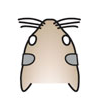
\includegraphics[width = 1.5 cm]{Diagrams/Presentation/indepears.png}\\
    \underline{\textbf{Independent Ears}}
    \small
     \begin{itemize}
    \item[] Eustachian tubes typically very narrow.
     \item[] Effectively independent eardrum vibrations.
     \end{itemize}
    \end{column}
     
    \begin{column}{0.5\textwidth}
    \centering
    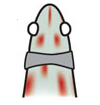
\includegraphics[width = 1.5 cm]{Diagrams/Presentation/coupledears.png}\\
    \underline{\textbf{Coupled Ears}}
    \small
     \begin{itemize}
         \item[] Eardrums connected through wide eustachian tubes and a large mouth cavity.
     \item[] Eardrums vibrations influence eachother.
     \end{itemize}
    \end{column}
    
  \end{columns}
  
\end{frame}

\begin{frame}
 \begin{exampleblock}{Advantages of Low Frequency Hearing}
  
 \end{exampleblock}

\end{frame}

\section{The Model}

\subsection{Mouth Cavity}
\begin{frame}[t]
\frametitle{Mouth Cavity}
% \begin{figure}[htl]
% \flushleft
% 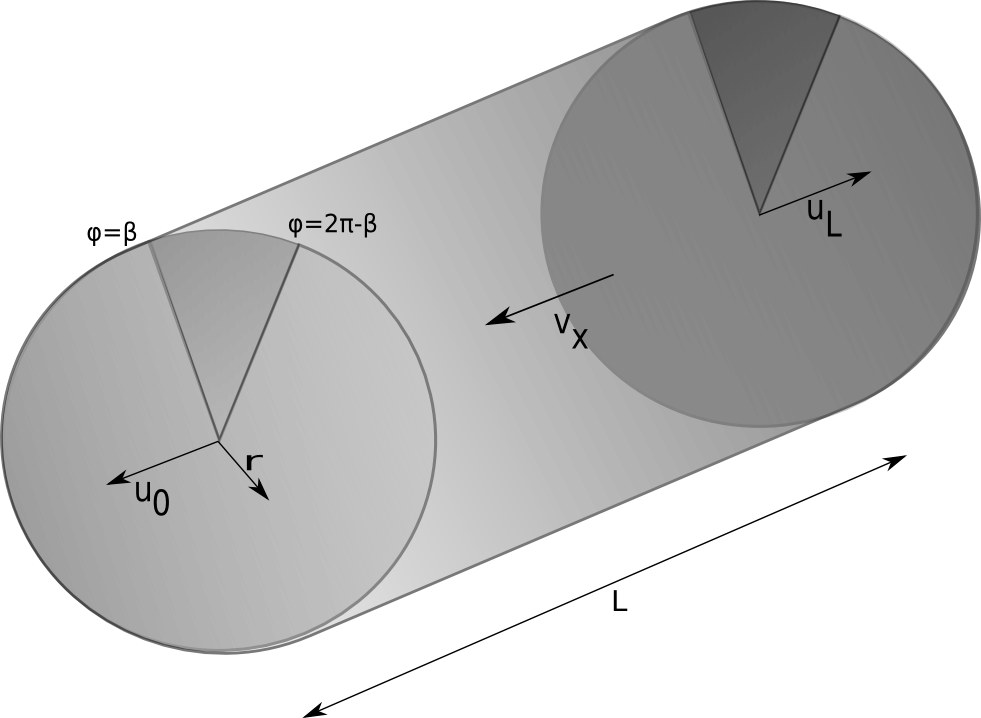
\includegraphics[width=.36\textwidth]{Diagrams/oldCylinder.png}
% %\caption{Previous Cylindrical Cavity}
% \end{figure}
% \begin{figure}[htr]
% 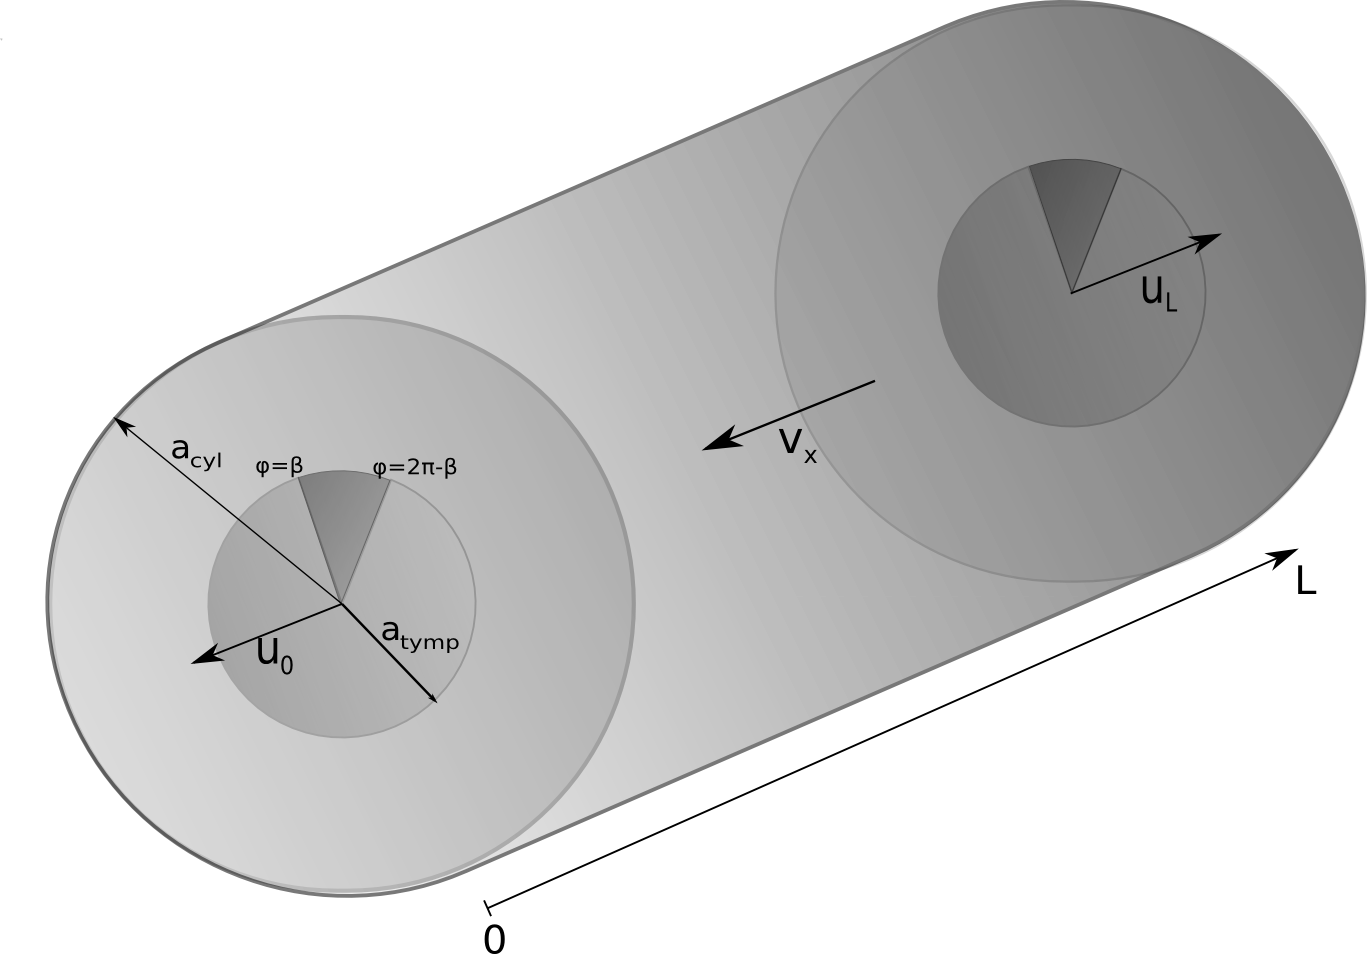
\includegraphics[width=.38\textwidth]{Diagrams/newCylinder.png}
% \caption{Mouth Cavity Model}
% \end{figure}
\begin{columns}

 \begin{column}{0.5\textwidth}
   \onslide<1->{
   \footnotesize
    \underline{\textbf{Previous Model}}\\
    \centering
    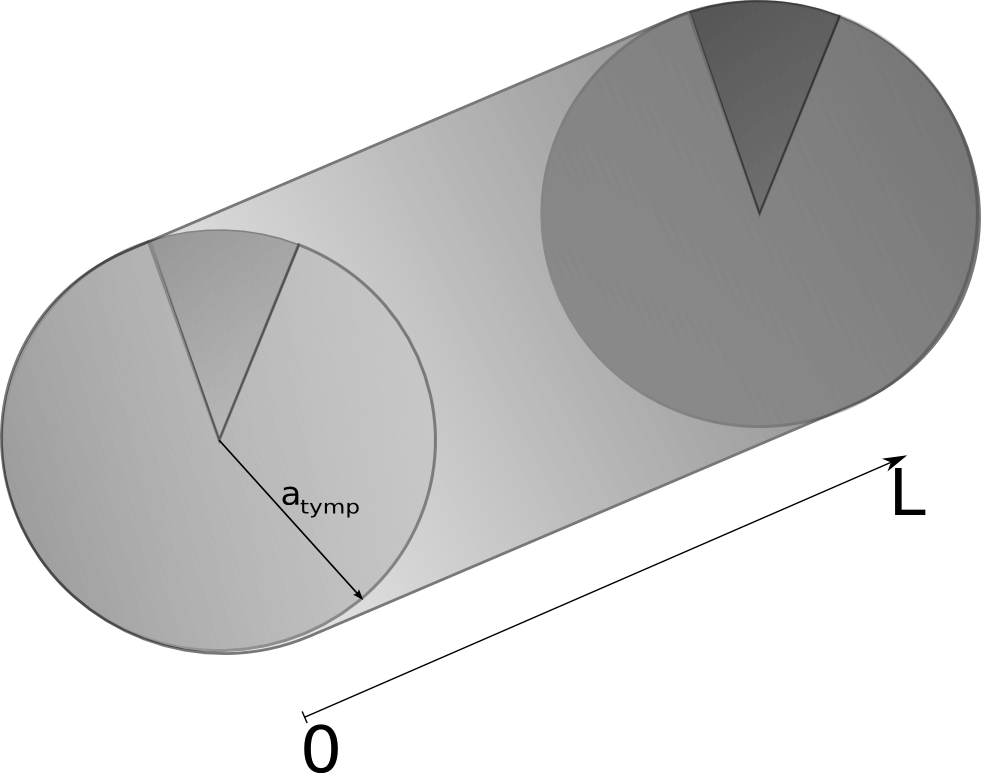
\includegraphics[width = 4 cm]{Diagrams/Presentation/oldCylinder.png}\\
    \small
    \begin{exampleblock}{ }
    \begin{itemize}
     \item[] $a_{\mathrm{tymp}}$ fixed.
     \item[] $V_{\mathrm{cyl}}=\pi a^2_{\mathrm{tymp}}L$
    \end{itemize}
    \end{exampleblock}}

    \end{column}
    
 \begin{column}{0.5\textwidth}
    \onslide<2->{
        \footnotesize
    \underline{\textbf{Our Model}}\\
    \centering
    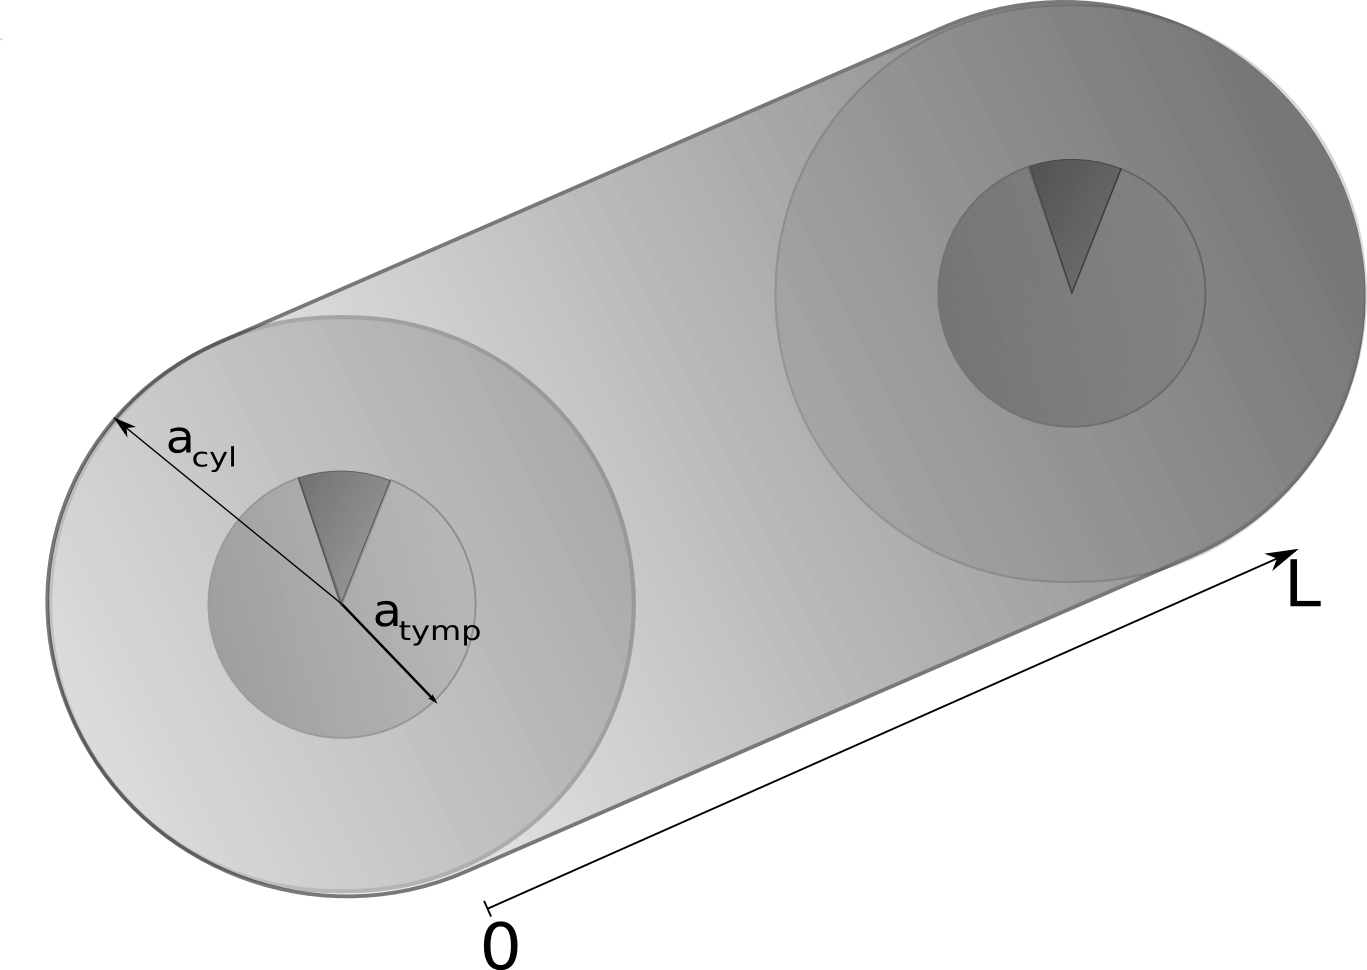
\includegraphics[width = 4 cm]{Diagrams/Presentation/newCylinder.png}\\
    \small
    \begin{exampleblock}{ }
    \begin{itemize}
     \item[] $a_{\mathrm{tymp}},\ V_{\mathrm{cyl}}$ fixed. 
     \item[] $a_{\mathrm{cyl}}=\sqrt{V_{\mathrm{cyl}}/\pi L}$
    \end{itemize}
    \end{exampleblock}}
    \end{column}
    
    \end{columns}
\end{frame}

\begin{frame}[t]
 \frametitle{Acoustic Head Model}
 \begin{columns}
     \begin{column}{.5\textwidth}
    \small
    \flushleft
     \onslide<1>{\begin{itemize}
      \item<1-> \textbf{I} - Ipsilateral ear, \textbf{C} - Contralateral ear.
      \item<1->  $p_0,\ p_L$ - sound pressure on eardrums,
      $\theta$ - sound source direction.
     \end{itemize}}
     
     \begin{itemize}
      \item<2-> Sound source ``far away''.
      \item<2-> Phase difference between sound at both ears - $\Delta=1.5kL\sin\theta$.
      \item<2-> No appreciable amplitude difference, $|p_0|=|p_L|$.
      \end{itemize}

    \end{column}
    
 \begin{column}{0.5\textwidth}
%     \centering
%     \small
%     \underline{\textbf{Head Model}}\\
%     \flushleft
    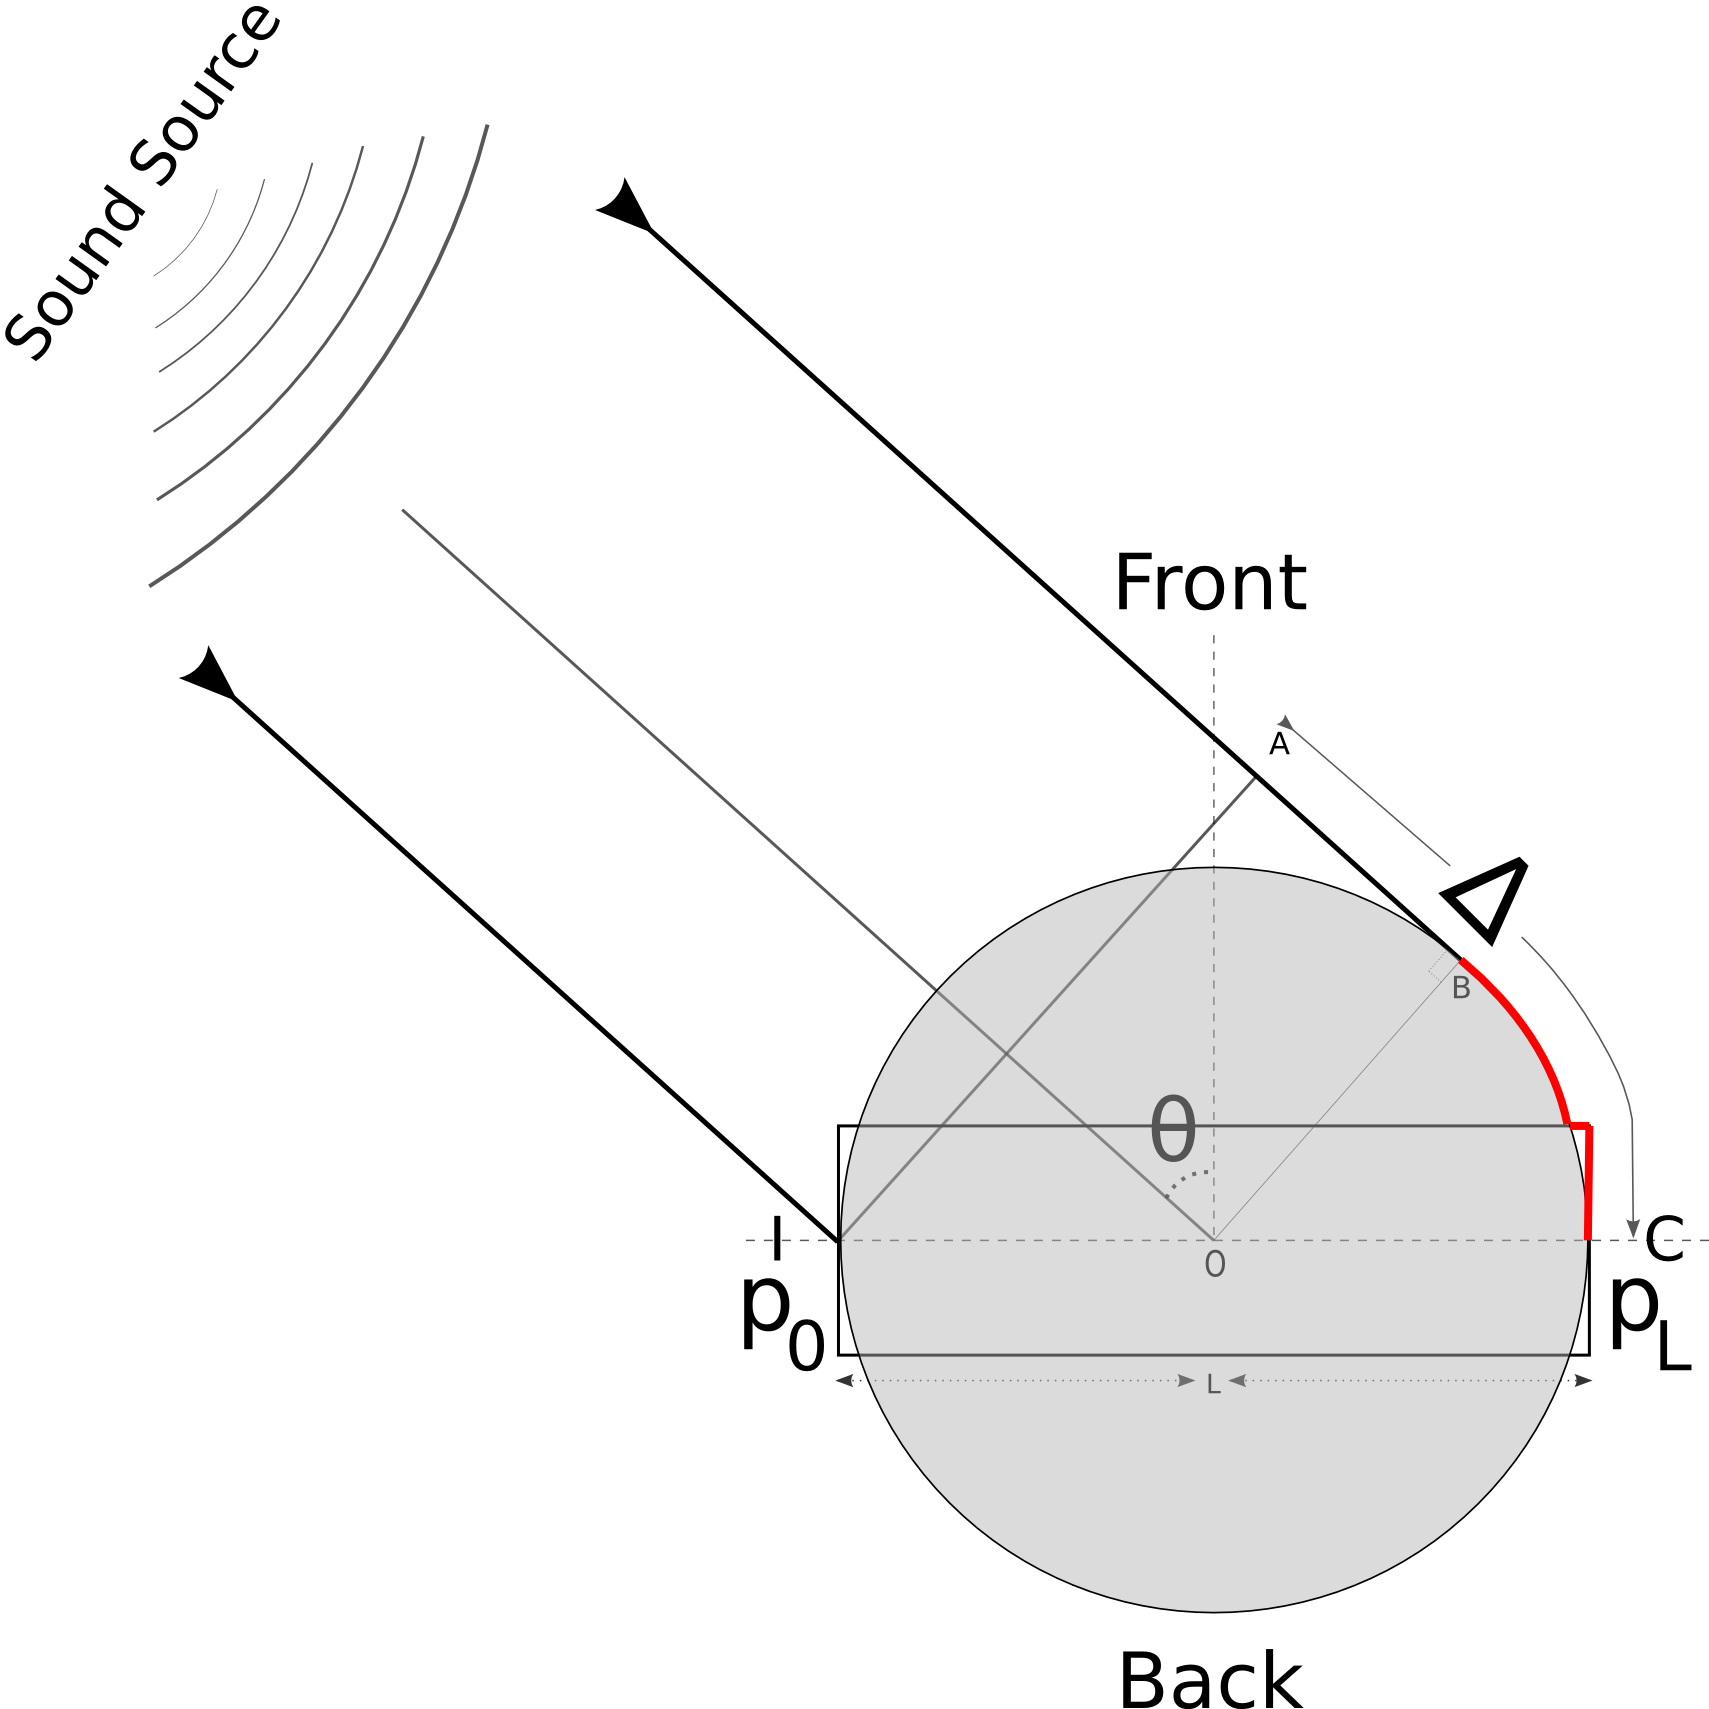
\includegraphics[width = 6 cm]{Diagrams/Presentation/acousticheadmodel2.png}\\
    \end{column}

    \end{columns}
\end{frame}


\begin{frame}
\frametitle{Cavity Pressure}
\begin{exampleblock}{3D Wave Equation}
\begin{equation}\label{pressurewaveeqn}
\begin{split}
 \frac{1}{c^2}\partial^2_t p(x,r,\phi,t)=\frac{1}{r}\frac{\partial}{\partial r}&\left(r\frac{\partial p(x,r,\phi,t)}{\partial r}\right)
 \\&+\frac{1}{r^2}\frac{\partial^2 p(x,r,\phi,t)}{\partial \phi^2}
 +\frac{\partial p(x,r,\phi,t)}{\partial x^2}
 \end{split}
\end{equation}
\end{exampleblock}
\begin{block}{}
 To be solved using the separation ansatz \[p(x,r,\phi,t)=f(x)g(r)h(\phi)e^{j\omega t}\].
\end{block}

% Subject to the no-penetration boundary condition at all solid boundaries.

\end{frame}

% \begin{frame}
% \frametitle{Eardrum}
% %  \begin{figure}[ht!]
% %   \centering
% %   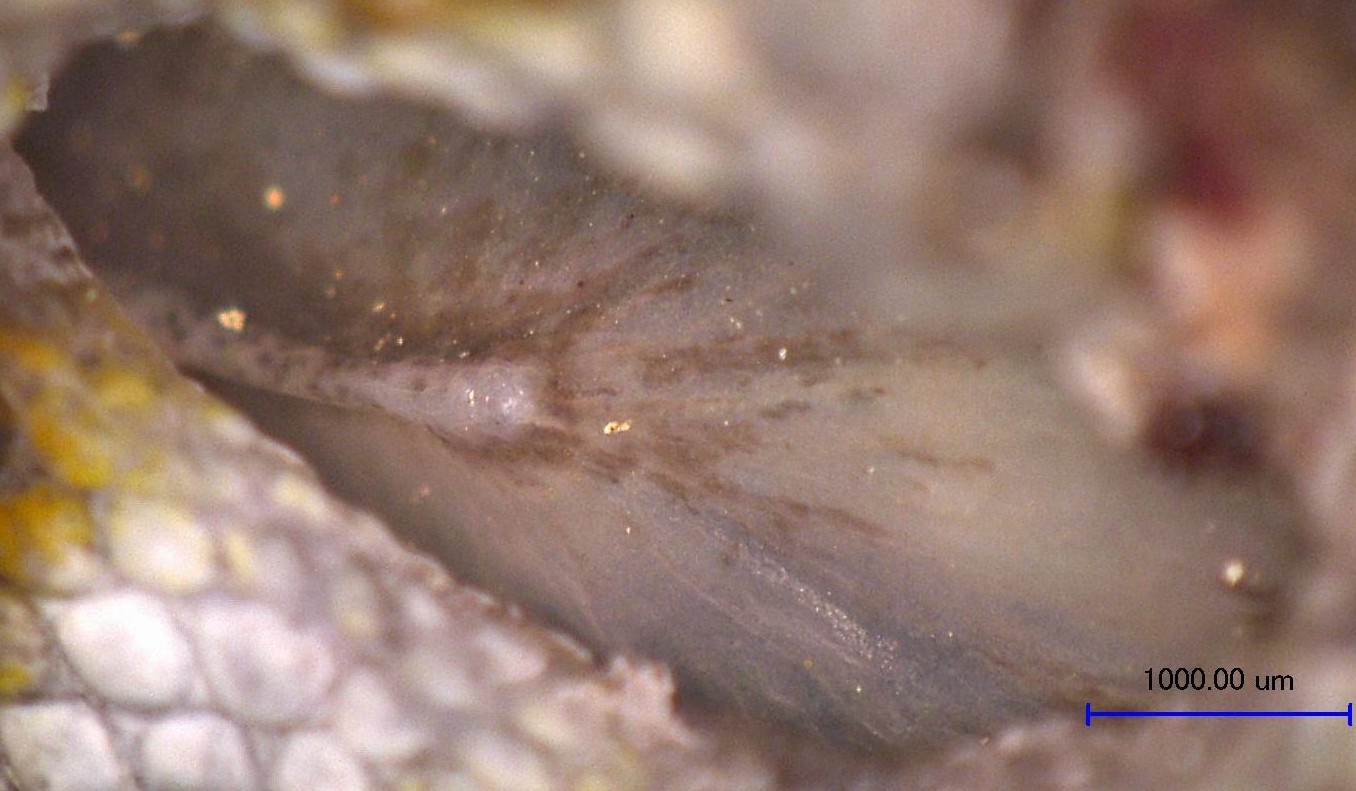
\includegraphics[width=.34\textwidth]{Diagrams/geckoextracolumella2.jpg}
% % \end{figure}
% \begin{figure}[htb!]
% \makebox[\linewidth]{
% 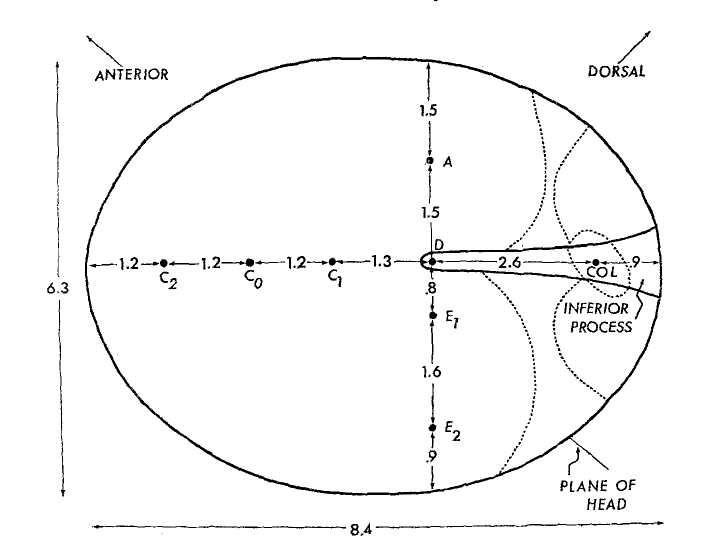
\includegraphics[width=.37\textwidth]{Diagrams/geckoear.png}
% \hfill
% 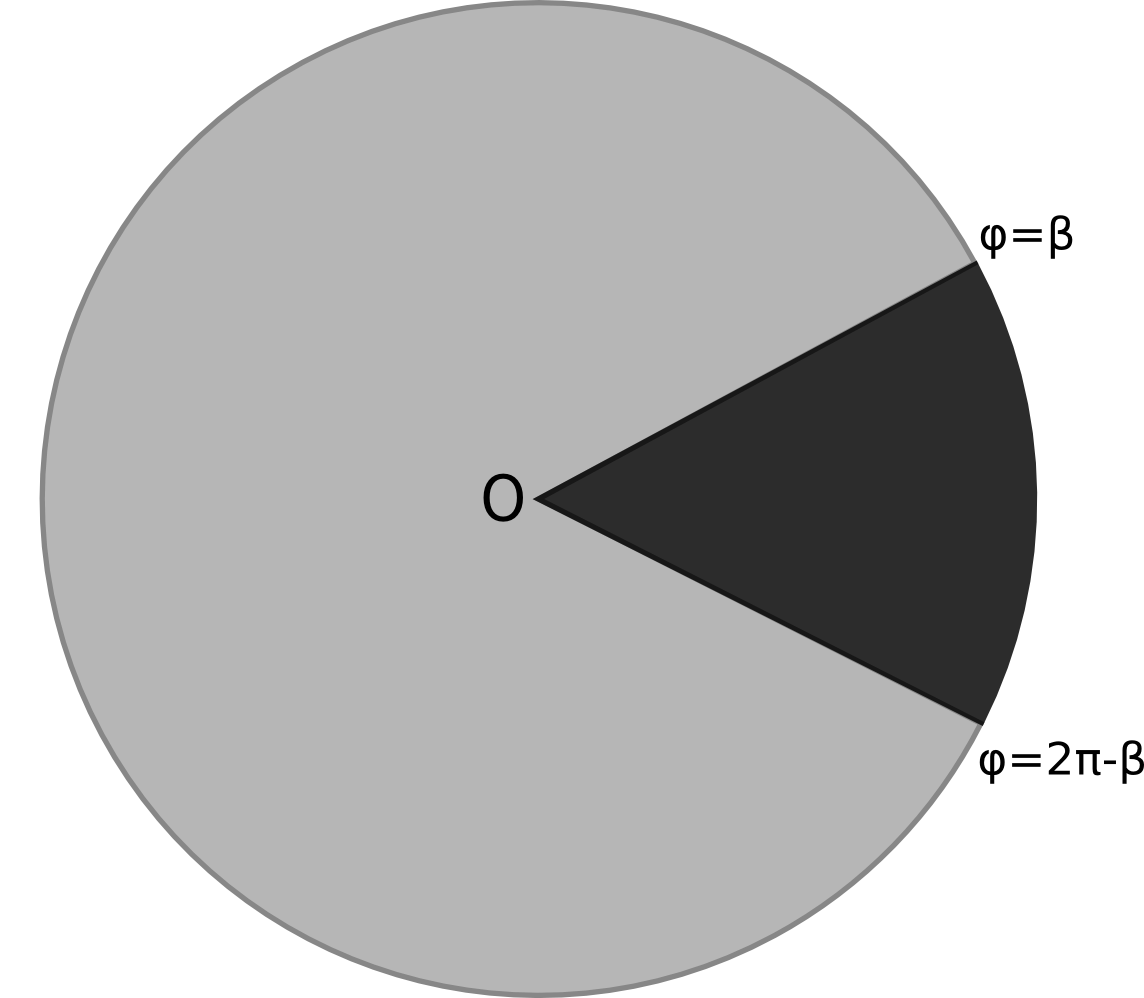
\includegraphics[width=.3\textwidth]{Diagrams/tympanummodel.png}}
% 
% \end{figure}
% 
% \end{frame}

\begin{frame}

\onslide<1->{\begin{block}{No-penetration at the cavity boundary, i.e. normal derivative vanishes}
\begin{equation}
 -j\rho\omega\mathbf{v}=\mathbf{n}.\left.\nabla p(x,r,\phi;t)\right|_{r=a_{\mathrm{cyl}}}=\left.\frac{\partial p}{\partial r}\right|_{r=a_{\mathrm{cyl}}}=0
\end{equation}
\end{block}}

 \onslide<2->{\begin{exampleblock}{Pressure Modes}
  \begin{align}
   &p_{\mathrm{qs}}(x,r,\phi;t)=\left[A_{\mathrm{qs}}e^{j\zeta_{\mathrm{qs}}x}+B_{qs}e^{-j\zeta_{\mathrm{qs}}x}\right]\cos q\phi J_q(\nu_{qs}r)e^{j\omega t}\\
   &\mbox{such that, }\quad \left.\frac{\partial J_q(\nu_{qs}r)}{\partial r}\right|_{r=a_{\mathrm{cyl}}}=0\quad\mbox{ and }\quad\zeta_{\mathrm{qs}}=\sqrt{k^2-\nu^2_{qs}}\nonumber
  \end{align}

 \end{exampleblock}}

\end{frame}

\begin{frame}
\begin{exampleblock}{Plane Wave Mode}
 \begin{equation}
  p_{\mathrm{00}}(x,r,\phi;t)=\left[Ae^{jkx}+B_{qs}e^{-jkx}\right]e^{j\omega t}
 \end{equation}
\end{exampleblock}
\begin{itemize}
 \item[] Trivially satisfies the no-penetration condition.
\end{itemize}

\end{frame}

\begin{frame}
\frametitle{Eardrum}
\begin{columns}
    \begin{column}{0.5\textwidth}
      \centering
      \small
      Sketch of a Tokay eardrum as seen from the outside\footnote{\bibentry{manleygecko1}}.\\
      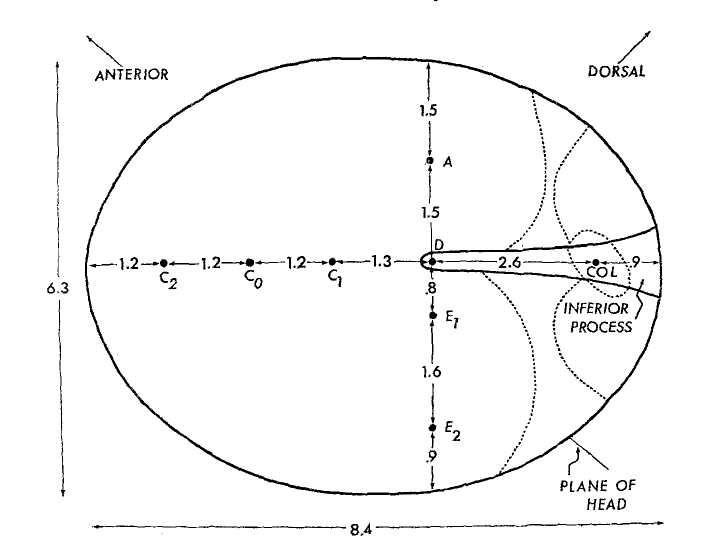
\includegraphics[width = 3.7 cm]{Diagrams/geckoear.png}\\
      \footnotesize
     COL - approximate position opposite the extracolumella insertion.
    \end{column}

    \begin{column}{0.5\textwidth}
      \centering
      \small
      The ICE eardrum.\\
      \textbf{}\\
      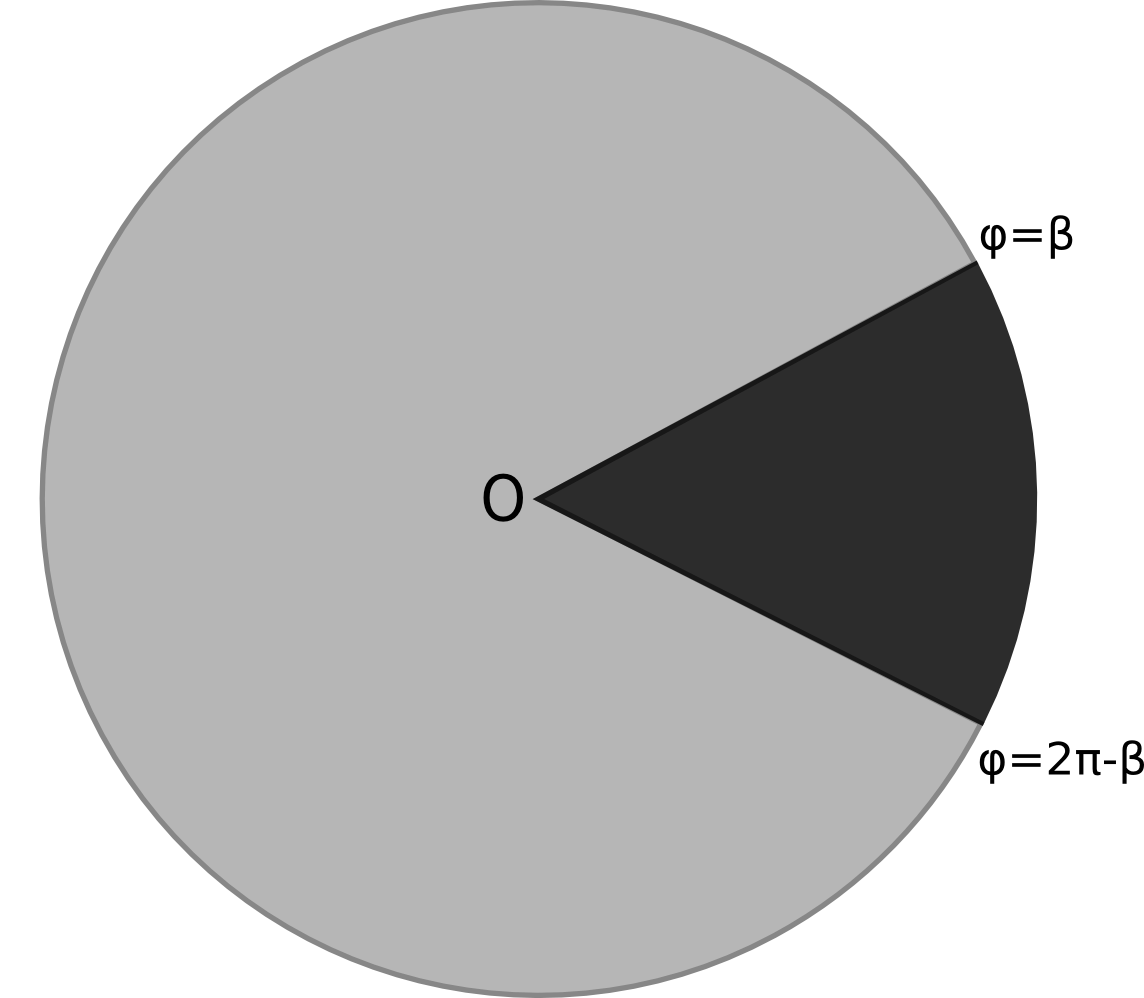
\includegraphics[width = 3.2 cm]{Diagrams/tympanummodel.png}\\
%       \textbf{}\\
%       Extracolumella (dark region) is rigid and stationary.\\
%       \textbf{}\\
%       The membrane material is assumed to be linear elastic.
\footnotesize
\begin{itemize}
      \item[] Extracolumella (dark) - rigid, stationary.
      \item[] Tympanum - assumed linear elastic.
      \item[] Rigidly clamped at the boundaries ($r=a_{\mathrm{tymp}}$ and $\phi=\beta,\ 2\pi-\beta$)
\end{itemize}

    \end{column}
  \end{columns}
  
\end{frame}


\begin{frame}
 \frametitle{Membrane Vibrations}
\onslide<1->{\begin{exampleblock}{Membrane EOM}

\begin{equation}\label{membraneequation1}
\begin{split}
 -\partial^2_tu(r,\phi;t)-2\alpha\partial_t u(r,\phi;t)+c^2_M\Delta_{(2)}&u(r,\phi;t)=\\ 
 & \frac{1}{\rho_m d}\Psi(r,\phi;t)
 \end{split}
\end{equation}
 \end{exampleblock}}

 \onslide<2->{\begin{block}{Membrane parameters}
  \begin{tabular}{l l}
    $\alpha$ - damping coefficient, & $c^2_M$ - propagation velocity\\
    $\rho_m$ - density, & $d$ - thickness.
  \end{tabular}
 \end{block}}

\end{frame}


\section{Evaluation}
\begin{frame}
\begin{columns}
    \begin{column}{0.5\textwidth}
      \centering
      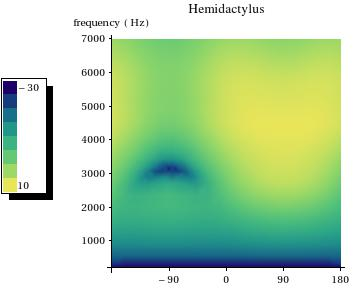
\includegraphics[width = 5.6 cm]{Diagrams/Plots/hemidactylusvibamp.jpeg}\\
    \end{column}

    \begin{column}{0.5\textwidth}
    \textbf{}\\
    %\textbf{}\\
    \vspace{1pt}
    \flushright
      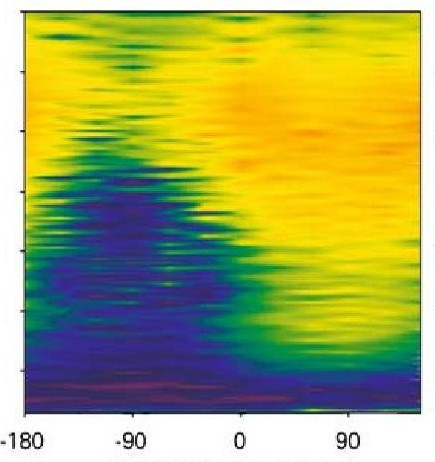
\includegraphics[width = 3.3 cm]{Diagrams/Plots/hemidactylusvibamp_exp.jpeg}
    \end{column}
  \end{columns}
\end{frame}

\section{Conclusion}
\begin{frame}
 Conclusion
\end{frame}

\begin{frame}
 \frametitle{Thank You}
 \begin{figure}
  \centering
  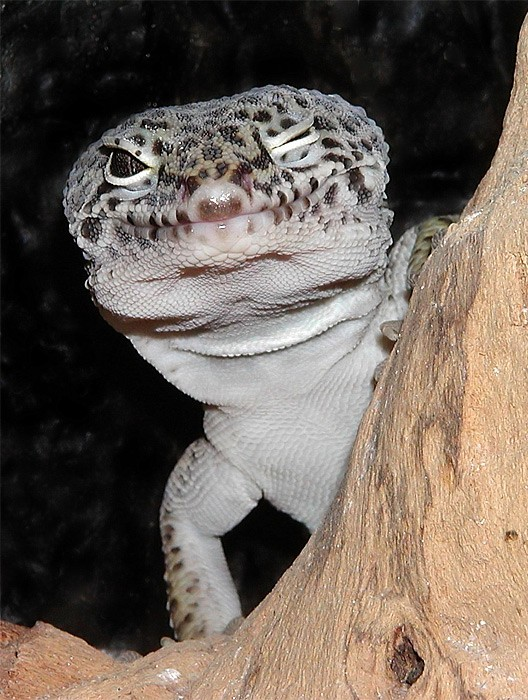
\includegraphics[width=.3\textwidth]{Diagrams/geckowink.jpg}
 \end{figure}
\end{frame}


\end{document}
